\documentclass[handout,noauthor,nooutcomes]{../ximera}

\graphicspath{  
{./}
{./whoAreYou/}
{./drawingWithTheTurtle/}
{./bisectionMethod/}
{./circles/}
{./anglesAndRightTriangles/}
{./lawOfSines/}
{./lawOfCosines/}
{./plotter/}
{./staircases/}
{./pitch/}
{./qualityControl/}
{./symmetry/}
{./nGonBlock/}
}


%% page layout
\usepackage[cm,headings]{fullpage}
\raggedright
\setlength\headheight{13.6pt}


%% fonts
\usepackage{euler}

\usepackage{FiraMono}
\renewcommand\familydefault{\ttdefault} 
\usepackage[defaultmathsizes]{mathastext}
\usepackage[htt]{hyphenat}

\usepackage[T1]{fontenc}
\usepackage[scaled=1]{FiraSans}

%\usepackage{wedn}
\usepackage{pbsi} %% Answer font


\usepackage{cancel} %% strike through in pitch/pitch.tex


%% \usepackage{ulem} %% 
%% \renewcommand{\ULthickness}{2pt}% changes underline thickness

\tikzset{>=stealth}

\usepackage{adjustbox}

\setcounter{titlenumber}{-1}

%% journal style
\makeatletter
\newcommand\journalstyle{%
  \def\activitystyle{activity-chapter}
  \def\maketitle{%
    \addtocounter{titlenumber}{1}%
                {\flushleft\small\sffamily\bfseries\@pretitle\par\vspace{-1.5em}}%
                {\flushleft\LARGE\sffamily\bfseries\thetitlenumber\hspace{1em}\@title \par }%
                {\vskip .6em\noindent\textit\theabstract\setcounter{question}{0}\setcounter{sectiontitlenumber}{0}}%
                    \par\vspace{2em}
                    \phantomsection\addcontentsline{toc}{section}{\thetitlenumber\hspace{1em}\textbf{\@title}}%
                     }}
\makeatother



%% thm like environments
\let\question\relax
\let\endquestion\relax

\newtheoremstyle{QuestionStyle}{\topsep}{\topsep}%%% space between body and thm
		{}                      %%% Thm body font
		{}                              %%% Indent amount (empty = no indent)
		{\bfseries}            %%% Thm head font
		{)}                              %%% Punctuation after thm head
		{ }                           %%% Space after thm head
		{\thmnumber{#2}\thmnote{ \bfseries(#3)}}%%% Thm head spec
\theoremstyle{QuestionStyle}
\newtheorem{question}{}



\let\freeResponse\relax
\let\endfreeResponse\relax

%% \newtheoremstyle{ResponseStyle}{\topsep}{\topsep}%%% space between body and thm
%% 		{\wedn\bfseries}                      %%% Thm body font
%% 		{}                              %%% Indent amount (empty = no indent)
%% 		{\wedn\bfseries}            %%% Thm head font
%% 		{}                              %%% Punctuation after thm head
%% 		{3ex}                           %%% Space after thm head
%% 		{\underline{\underline{\thmname{#1}}}}%%% Thm head spec
%% \theoremstyle{ResponseStyle}

\usepackage[tikz]{mdframed}
\mdfdefinestyle{ResponseStyle}{leftmargin=1cm,linecolor=black,roundcorner=5pt,
, font=\bsifamily,}%font=\wedn\bfseries\upshape,}


\ifhandout
\NewEnviron{freeResponse}{}
\else
%\newtheorem{freeResponse}{Response:}
\newenvironment{freeResponse}{\begin{mdframed}[style=ResponseStyle]}{\end{mdframed}}
\fi



%% attempting to automate outcomes.

%% \newwrite\outcomefile
%%   \immediate\openout\outcomefile=\jobname.oc
%% \renewcommand{\outcome}[1]{\edef\theoutcomes{\theoutcomes #1~}%
%% \immediate\write\outcomefile{\unexpanded{\outcome}{#1}}}

%% \newcommand{\outcomelist}{\begin{itemize}\theoutcomes\end{itemize}}

%% \NewEnviron{listOutcomes}{\small\sffamily
%% After answering the following questions, students should be able to:
%% \begin{itemize}
%% \BODY
%% \end{itemize}
%% }
\usepackage[tikz]{mdframed}
\mdfdefinestyle{OutcomeStyle}{leftmargin=2cm,rightmargin=2cm,linecolor=black,roundcorner=5pt,
, font=\small\sffamily,}%font=\wedn\bfseries\upshape,}
\newenvironment{listOutcomes}{\begin{mdframed}[style=OutcomeStyle]After answering the following questions, students should be able to:\begin{itemize}}{\end{itemize}\end{mdframed}}



%% my commands

\newcommand{\snap}{{\bfseries\itshape\textsf{Snap!}}}
\newcommand{\flavor}{\link[\snap]{https://snap.berkeley.edu/}}
\newcommand{\mooculus}{\textsf{\textbf{MOOC}\textnormal{\textsf{ULUS}}}}


\usepackage{tkz-euclide}
\tikzstyle geometryDiagrams=[rounded corners=.5pt,ultra thick,color=black]
\colorlet{penColor}{black} % Color of a curve in a plot



\ifhandout\newcommand{\mynewpage}{\newpage}\else\newcommand{\mynewpage}{}\fi


\title{Drawing with the turtle}
\author{Bart Snapp}

\begin{document}
\begin{abstract}
  We will use \snap\ to draw things.
\end{abstract}
\maketitle

\begin{listOutcomes}
\item{Use \snap\ blocks to form a basic \snap\ script.}
\item{Know the terms \textbf{script} and \textbf{stage} in reference to \snap\ programming.}
\item{Direct the \snap\ turtle to draw pictures.}
\item{Recover basic geometry facts through personal research.}
\item{Use the \textbf{repeat} command to automated repeated processes.}
\item{Recognize that identifying a triangle based on minimal
  congruence properties requires nontrivial work.}
\end{listOutcomes}

\begin{listObjectives}
 \item Learn and apply basic geometric formulas,
 \item Take a solution to a problem in a given context, and applying that same solution to another problem,
\item Increase student confidence in their ability to solve difficult math problems by using previous results, trying different methods, asking questions, and working with others.
\end{listObjectives}

\snap\ is a fun programming language where you help a \textbf{drawing
  turtle} create beautiful pictures.  Here is what that artistic
turtle looks like:
\raisebox{-.3\height}{
\includegraphics{turtle.png}}.


To guide the turtle around, you assemble blocks into
\snap\ \textbf{scripts} like so:

 \adjustbox{valign=t}{
   \begin{tabular}{lp{.7\textwidth}}
      \raisebox{-\height}{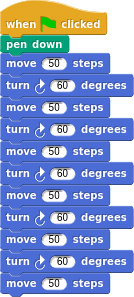
\includegraphics{hex-script.png}} &

This will make the turtle draw a picture on the \textbf{stage}.  Once
you draw stuff, you might want to start over. To do this, use:
\begin{center}
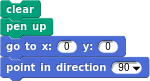
\includegraphics{clear-script.png}
\end{center}
   \end{tabular}}
\mynewpage


\begin{question}
  Use \snap\ to draw:
  \begin{enumerate}
  \item A rectangle with side lengths $50$ and $100$.
  \item An equilateral triangle of side length $100$.
  \item A regular pentagon of side length $50$.
  \end{enumerate}
  Show off your work by giving screenshots of your SCRIPTS and STAGES
  as provided from \snap.
  \begin{freeResponse}
    \begin{enumerate}
    \item Here is my script and my stage for the rectangle:
      \begin{center}
        \raisebox{-.2\height}{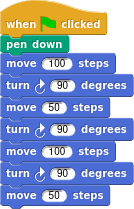
\includegraphics{firstRectangle-script.png}}
        \qquad
        \fbox{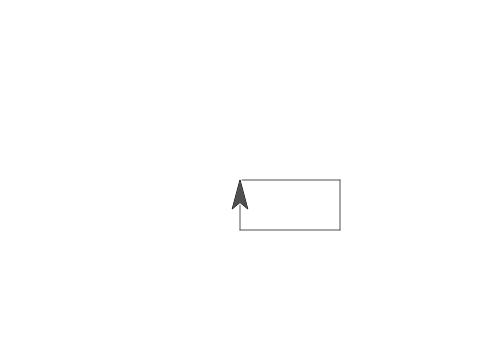
\includegraphics[width=.4\textwidth]{firstRectangle-stage.png}}
      \end{center}
    \item Here is my script and my stage for the triangle:
      \begin{center}
        \raisebox{-.2\height}{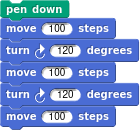
\includegraphics{firstTriangle-script.png}}
        \qquad
        \fbox{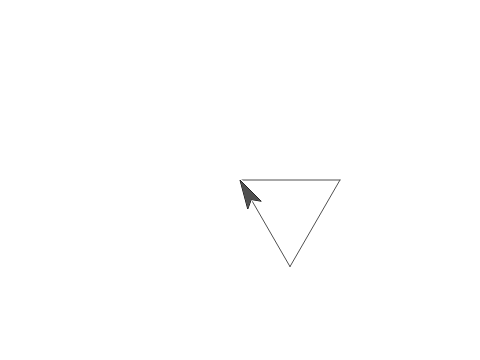
\includegraphics[width=.4\textwidth]{firstTriangle-stage.png}}
      \end{center}
    \item Here is my script and my stage for the pentagon:
      \begin{center}
        \raisebox{-.2\height}{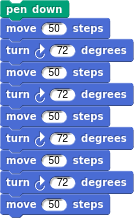
\includegraphics{firstPentagon-script.png}}
        \qquad
        \fbox{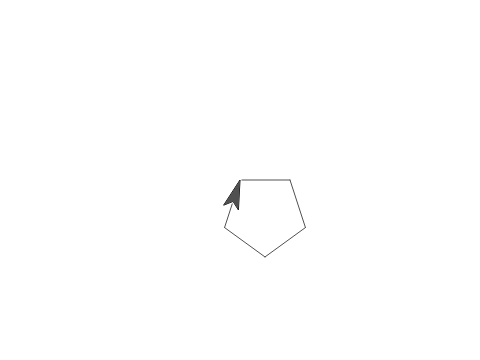
\includegraphics[width=.4\textwidth]{firstPentagon-stage.png}}
      \end{center}
    \end{enumerate}
  \end{freeResponse}
\end{question}
\mynewpage

\begin{question}
  If you think about the scripts above, you'll see that we repeated
  ourselves a lot. We can make this easier with the \textbf{repeat block}:
  \begin{center}
    
\includegraphics{repeat-block.png}
  \end{center}
  Use the repeat block to help draw:
  \begin{enumerate}
  \item An equilateral triangle of side length $100$.
  \item A regular pentagon of side length $50$.
  \item A regular $17$-gon of side length $30$.
  \end{enumerate}
  Show off your work by giving screenshots of your SCRIPTS and STAGES
  as provided from \snap.
    \begin{freeResponse}
    \begin{enumerate}
    \item Here is my script and stage for the triangle:
      \begin{center}
        \raisebox{-.2\height}{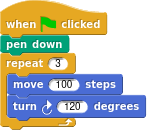
\includegraphics{secondTriangle-script.png}}
        \qquad
        \fbox{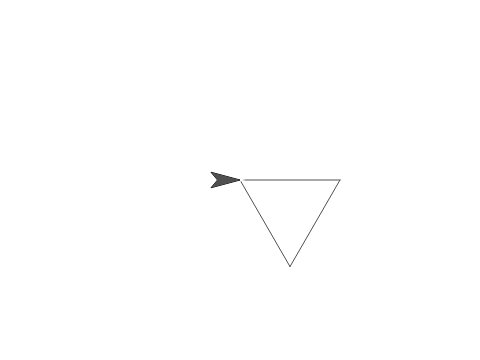
\includegraphics[width=.4\textwidth]{secondTriangle-stage.png}}
      \end{center}
    \item Here is my script and stage for the pentagon:
      \begin{center}
        \raisebox{-.2\height}{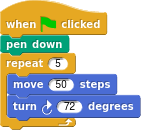
\includegraphics{secondPentagon-script.png}}
        \qquad
        \fbox{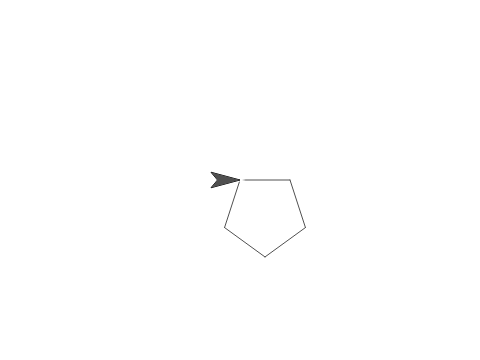
\includegraphics[width=.4\textwidth]{secondPentagon-stage.png}}
      \end{center}
    \item Here is my script and stage for the $17$-gon:
      \begin{center}
        \raisebox{-.2\height}{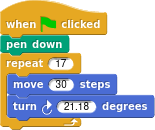
\includegraphics{repeat17gon-script.png}}
        \qquad
        \fbox{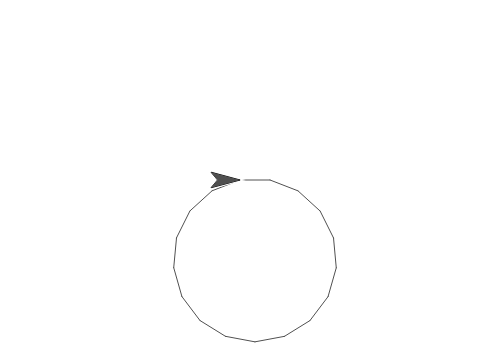
\includegraphics[width=.4\textwidth]{repeat17gon-stage.png}}
      \end{center}
    \end{enumerate}
  \end{freeResponse}
\end{question}
\mynewpage

\begin{question}
  Use \snap\ and the turtle to draw:
  \begin{enumerate}
  \item An isosceles right triangle, with legs of length $100$.
  \item A $30^\circ$-$60^\circ$-$90^\circ$ triangle, with shortest leg of length $50$.
  \item A triangle with side lengths: $90$, $120$, $150$.
  \end{enumerate}
  Show off your work by giving screenshots of your SCRIPTS and STAGES as
  provided from \snap.

  
  In each of these cases, there will be numbers that you need to find,
  either through calculations or INTERNET searches. EXPLAIN what
  numbers you needed and how you found them.
  
  \begin{freeResponse}
    \begin{enumerate}
    \item Here is my script and stage for the isosceles right
      triangle:
      \begin{center}
        \raisebox{-.2\height}{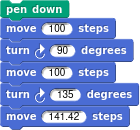
\includegraphics{isoscelesRightTri-script.png}}
        \qquad
        \fbox{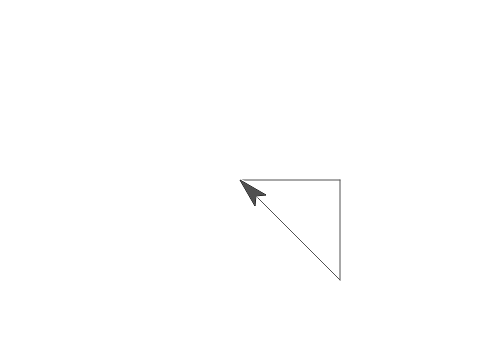
\includegraphics[width=.4\textwidth]{isoscelesRightTri-stage.png}}
      \end{center}
      Here I needed to figure out that the hypotenuse had length
      $141.42$. I found this with the Pythagorean theorem:
      \begin{align*}
      100^2 + 100^2 &= c^2\\
      c &= \sqrt{20000}\\
      c &\approx 141.42
      \end{align*}
      
    \item Here is my script and stage for the $30^\circ$-$60^\circ$-$90^\circ$ triangle:
      \begin{center}
        \raisebox{-.2\height}{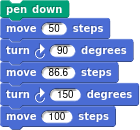
\includegraphics{306090-script.png}}
        \qquad
        \fbox{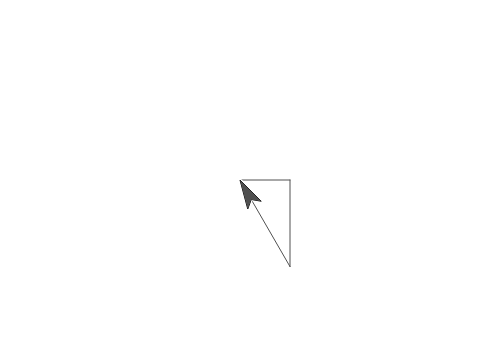
\includegraphics[width=.4\textwidth]{306090-stage.png}}
      \end{center}
      Here I needed to know that the hypotenuse is twice the length of
      the shortest leg, and to figure out that the longest leg had
      length $86.6$.  I found the length of of the longest leg with
      the Pythagorean theorem:
      \begin{align*}
      50^2 + b^2 &= 100^2\\
      b &= \sqrt{7500}\\
      b &\approx 86.6
      \end{align*}
    
    \item Here I needed to know that a $90$, $120$, $150$ triangle is
      just scaled $3:4:5$ right triangle. Using the INTERNET, I can
      find the angles.  Here is my script and stage:
      \begin{center}
        \raisebox{-.2\height}{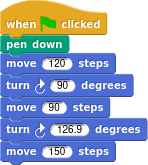
\includegraphics{90120150-script.png}}
        \qquad
        \fbox{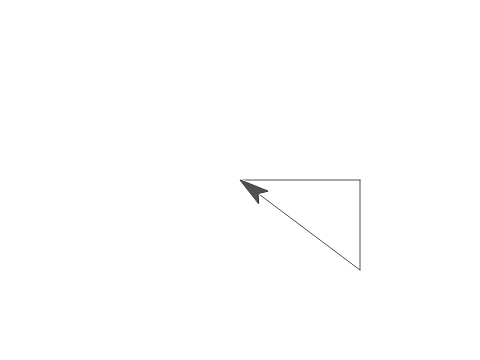
\includegraphics[width=.4\textwidth]{90120150-stage.png}}
      \end{center}
    \end{enumerate}
  \end{freeResponse}
\end{question}



\end{document}
